\documentclass{beamer}
\usepackage{tikz} % Figures
\usepackage{subcaption}
\usepackage{graphicx} % Images
% To write formulas
\usepackage{amsfonts}
\usepackage{amsmath}
\usepackage{caption}

\usetheme{Darmstadt}

\newcommand\tab[1][1cm]{\hspace*{#1}}

\makeatletter
\setbeamertemplate{title page}{
	\begin{centering}
		\begin{beamercolorbox}[sep=8pt,center]{institute}
			\usebeamerfont{institute}\insertinstitute
		\end{beamercolorbox}
		\begin{beamercolorbox}[sep=8pt,center]{title}
			\usebeamerfont{title}\inserttitle
		\end{beamercolorbox}
		\begin{beamercolorbox}[sep=8pt,center]{date}
			\usebeamerfont{author}\insertauthor \newline
			\usebeamerfont{date}\insertdate
		\end{beamercolorbox}
	\end{centering}
}
\makeatother
\title[Reducing Grenoble's car traffic]{\textsc{Decision Support System for carpooling to reduce car traffic in Grenoble area}}
\author{Romain NAVARRO}
\institute{ORCO \\ UGA \& ENSIMAG}
\date{June, 29\textsuperscript{th} 2018}


\AtBeginSection[]{%
	\begin{frame}<beamer>
		\frametitle{Outline}
		\tableofcontents[currentsection,hideallsubsections]
	\end{frame}
	\addtocounter{framenumber}{-1}% Don't affect slide number
}

\AtBeginSubsection[]{
	\begin{frame}<beamer>
		\frametitle{Outline}
		\tableofcontents[sectionstyle=show/hide,subsectionstyle=show/shaded/hide]
	\end{frame}
	\addtocounter{framenumber}{-1}% Don't affect slide number
}

\begin{document}
	\begin{frame}
		\maketitle
		\begin{tabbing}
			Supervisor:\tab \= \textsc{Prof.} \=Van-Dat \textsc{CUNG}, G-SCOP \& UGA\\\medskip
			Jury members: \> \textsc{Prof.} \>Nadia \textsc{BRAUNER}\\
			\> \textsc{Prof.} \>Van-Dat \textsc{CUNG}\\
			\> \textsc{Dr.} \>Vassilissa \textsc{LEHOUX}\\
			\> \textsc{Prof.} \>Matej \textsc{STEHLIK}
		\end{tabbing}
	\end{frame}
	
	\begin{frame}
		\tableofcontents[hideallsubsections]
	\end{frame}
	%%%%%%%%%%%%% DEF OF THE GOAL %%%%%%%%%%
	\section{Goal}
	\begin{frame}[label=pagebanale]
		\frametitle{Goal}
		\framesubtitle{Satisfaction of the users}
		\begin{itemize}
			\item Flexibility
			\item Schedules
			\item Detours
		\end{itemize}
		\footnotetext{references in the report}
	\end{frame}
	
	%%%%%%%%% PRESENTATION OF THE PROBLEM %%%%%%%%%%
	\section{Problem's presentation}
	\begin{frame}
		\frametitle{Presentation of the problem}
		\begin{figure}
			\centering
			\begin{subfigure}{.5\textwidth}
				\centering
				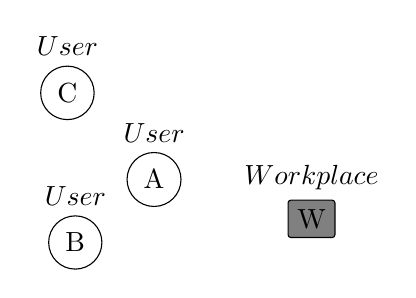
\begin{tikzpicture}
					\node[draw, circle, label=above:{$User$}] (A)at(-1.5, 0.5) {A};
					\node[draw, circle, label=above:{$User$}] (B)at(-2.5, -0.3) {B};
					\node[draw, circle, label=above:{$User$}] (C)at(-2.6, 1.6) {C};
					\node[draw, rectangle, rounded corners=1pt, fill=gray!100, label=above:{$Workplace$}] (W)at(0.5, 0) {W};
				\end{tikzpicture}
				\caption{User requests}
			\end{subfigure}%
			\begin{subfigure}{.5\textwidth}
				\centering
				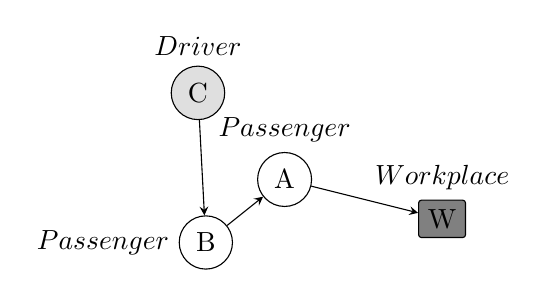
\begin{tikzpicture}
					\node[draw, circle, label=above:{$Passenger$}] (A)at(-1.5, 0.5) {A};
					\node[draw, circle, label=left:{$Passenger$}] (B)at(-2.5, -0.3) {B};
					\node[draw, circle, fill=gray!25, label=above:{$Driver$}] (C)at(-2.6, 1.6) {C};
					\node[draw, rectangle, rounded corners=1pt, fill=gray!100, label=above:{$Workplace$}] (W)at(0.5, 0) {W};
					\draw[->, >=stealth] (C) -- (B);
					\draw[->, >=stealth] (B) -- (A);
					\draw[->, >=stealth] (A) -- (W);
				\end{tikzpicture}
				\caption{A solution}
			\end{subfigure}
			\caption{Same workplace}
			\label{fig:same workplace}
		\end{figure}
	\end{frame}
	\subsection{Different workplaces}
	\begin{frame}
		\frametitle{Presentation of the problem}
		\framesubtitle{Different workplaces}
		\begin{figure}
			\centering
			\begin{subfigure}{.5\textwidth}
				\centering
				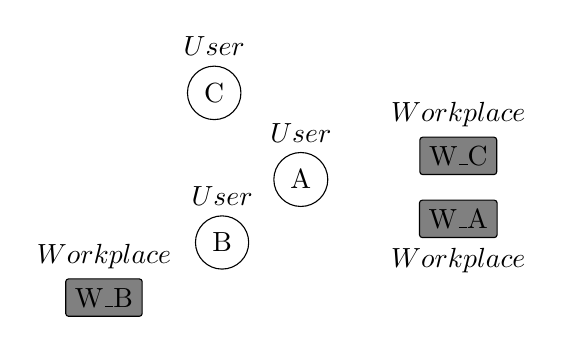
\begin{tikzpicture}
					\node[draw, circle, label=above:{$User$}] (A)at(-1.5, 0.5) {A};
					\node[draw, circle, label=above:{$User$}] (B)at(-2.5, -0.3) {B};
					\node[draw, circle, label=above:{$User$}] (C)at(-2.6, 1.6) {C};
					\node[draw, rectangle, rounded corners=1pt, fill=gray!100, label=below:{$Workplace$}] (WA)at(0.5, 0) {W\_A};
					\node[draw, rectangle, rounded corners=1pt, fill=gray!100, label=above:{$Workplace$}] (WC)at(0.5, 0.8) {W\_C};
					\node[draw, rectangle, rounded corners=1pt, fill=gray!100, label=above:{$Workplace$}] (WB)at(-4, -1) {W\_B};
				\end{tikzpicture}
				\caption{User requests}
			\end{subfigure}%
			\begin{subfigure}{.5\textwidth}
				\centering
				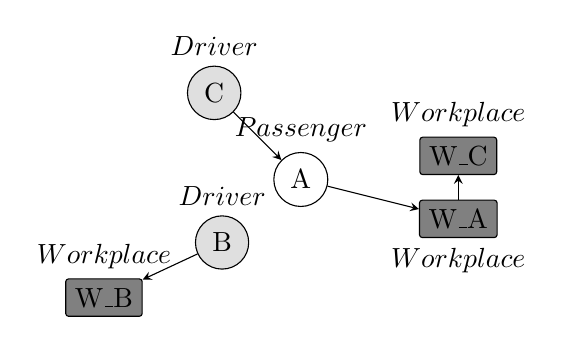
\begin{tikzpicture}
					\node[draw, circle, label=above:{$Passenger$}] (A)at(-1.5, 0.5) {A};
					\node[draw, circle, fill=gray!25, label=above:{$Driver$}] (B)at(-2.5, -0.3) {B};
					\node[draw, circle, fill=gray!25, label=above:{$Driver$}] (C)at(-2.6, 1.6) {C};
					\node[draw, rectangle, rounded corners=1pt, fill=gray!100, label=below:{$Workplace$}] (WA)at(0.5, 0) {W\_A};
					\node[draw, rectangle, rounded corners=1pt, fill=gray!100, label=above:{$Workplace$}] (WC)at(0.5, 0.8) {W\_C};
					\node[draw, rectangle, rounded corners=1pt, fill=gray!100, label=above:{$Workplace$}] (WB)at(-4, -1) {W\_B};
					\draw[->, >=stealth] (C) -- (A);
					\draw[->, >=stealth] (A) -- (WA);
					\draw[->, >=stealth] (WA) -- (WC);
					\draw[->, >=stealth] (B) -- (WB);
				\end{tikzpicture}
				\caption{A solution}
			\end{subfigure}
			\caption{Different workplaces}
			\label{fig:different workplaces}
		\end{figure}
	\end{frame}
	\subsection{Time windows}
	\begin{frame}
		\frametitle{Presentation of the problem}
		\framesubtitle{Time windows}
		\begin{figure}
			\centering
			\begin{subfigure}{.5\textwidth}
				\centering
				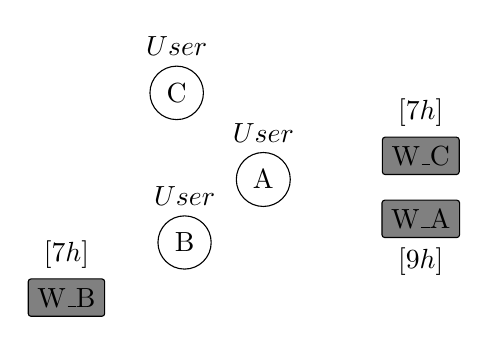
\begin{tikzpicture}
					\node[draw, circle, label=above:{$User$}] (A)at(-1.5, 0.5) {A};
					\node[draw, circle, label=above:{$User$}] (B)at(-2.5, -0.3) {B};
					\node[draw, circle, label=above:{$User$}] (C)at(-2.6, 1.6) {C};
					\node[draw, rectangle, rounded corners=1pt, fill=gray!100, label=below:{$[9h]$}] (WA)at(0.5, 0) {W\_A};
					\node[draw, rectangle, rounded corners=1pt, fill=gray!100, label=above:{$[7h]$}] (WC)at(0.5, 0.8) {W\_C};
					\node[draw, rectangle, rounded corners=1pt, fill=gray!100, label=above:{$[7h]$}] (WB)at(-4, -1) {W\_B};
				\end{tikzpicture}
				\caption{User requests}
			\end{subfigure}%
			\begin{subfigure}{.5\textwidth}
				\centering
				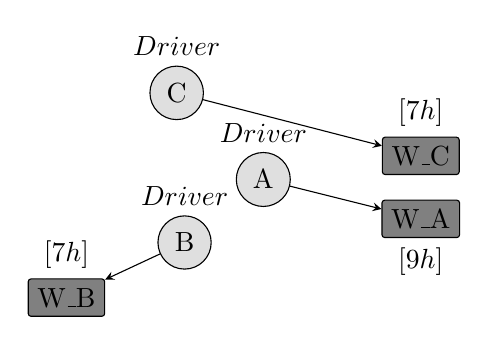
\begin{tikzpicture}
					\node[draw, circle, fill=gray!25, label=above:{$Driver$}] (A)at(-1.5, 0.5) {A};
					\node[draw, circle, fill=gray!25, label=above:{$Driver$}] (B)at(-2.5, -0.3) {B};
					\node[draw, circle, fill=gray!25, label=above:{$Driver$}] (C)at(-2.6, 1.6) {C};
					\node[draw, rectangle, rounded corners=1pt, fill=gray!100, label=below:{$[9h]$}] (WA)at(0.5, 0) {W\_A};
					\node[draw, rectangle, rounded corners=1pt, fill=gray!100, label=above:{$[7h]$}] (WC)at(0.5, 0.8) {W\_C};
					\node[draw, rectangle, rounded corners=1pt, fill=gray!100, label=above:{$[7h]$}] (WB)at(-4, -1) {W\_B};
					\draw[->, >=stealth] (C) -- (WC);
					\draw[->, >=stealth] (A) -- (WA);
					\draw[->, >=stealth] (B) -- (WB);
				\end{tikzpicture}
				\caption{A solution}
			\end{subfigure}
			\caption{Different time windows}
			\label{fig:different time windows}
		\end{figure}
	\end{frame}
	\subsection{Objective}
	\begin{frame}
		\frametitle{Presentation of the problem}
		\framesubtitle{Objective}
		\begin{figure}
			\centering
			\begin{subfigure}{.5\textwidth}
				\centering
				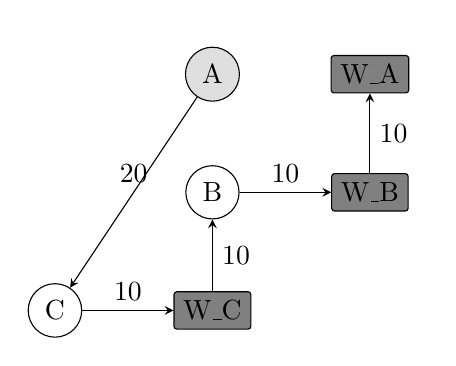
\begin{tikzpicture}
					\node[draw, circle, fill=gray!25, label=above:{$$}] (A)at(-1.5, 1) {A};
					\node[draw, circle, label=above:{$$}] (B)at(-1.5, -0.5) {B};
					\node[draw, circle, label=above:{$$}] (C)at(-3.5, -2) {C};
					\node[draw, rectangle, rounded corners=1pt, fill=gray!100, label=right:{$$}] (WA)at(0.5, 1) {W\_A};
					\node[draw, rectangle, rounded corners=1pt, fill=gray!100, label=right:{$$}] (WB)at(0.5, -0.5) {W\_B};
					\node[draw, rectangle, rounded corners=1pt, fill=gray!100, label=right:{$$}] (WC)at(-1.5, -2) {W\_C};
					\draw[->, >=stealth, above] (A) -- (C) node[midway] {$20$};
					\draw[->, >=stealth, above] (C) -- (WC) node[midway] {$10$};
					\draw[->, >=stealth, right] (WC) -- (B) node[midway] {$10$};
					\draw[->, >=stealth, above] (B) -- (WB) node[midway] {$10$};
					\draw[->, >=stealth, right] (WB) -- (WA) node[midway] {$10$};
				\end{tikzpicture}
				\caption{Total cost = 60}
			\end{subfigure}%
			\begin{subfigure}{.5\textwidth}
				\centering
				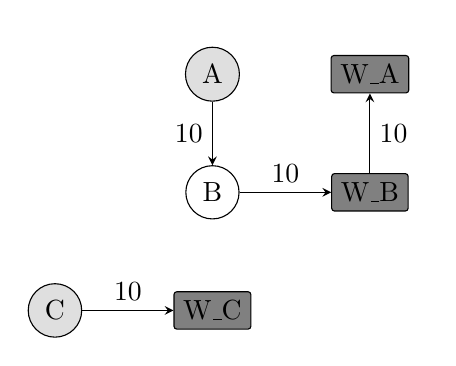
\begin{tikzpicture}
					\node[draw, circle, fill=gray!25, label=above:{$$}] (A)at(-1.5, 1) {A};
					\node[draw, circle, label=above:{$$}] (B)at(-1.5, -0.5) {B};
					\node[draw, circle, fill=gray!25, label=above:{$$}] (C)at(-3.5, -2) {C};
					\node[draw, rectangle, rounded corners=1pt, fill=gray!100, label=right:{$$}] (WA)at(0.5, 1) {W\_A};
					\node[draw, rectangle, rounded corners=1pt, fill=gray!100, label=right:{$$}] (WB)at(0.5, -0.5) {W\_B};
					\node[draw, rectangle, rounded corners=1pt, fill=gray!100, label=right:{$$}] (WC)at(-1.5, -2) {W\_C};
					\draw[->, >=stealth, left] (A) -- (B) node[midway] {$10$};
					\draw[->, >=stealth, above] (C) -- (WC) node[midway] {$10$};
					\draw[->, >=stealth, above] (B) -- (WB) node[midway] {$10$};
					\draw[->, >=stealth, right] (WB) -- (WA) node[midway] {$10$};
				\end{tikzpicture}
				\caption{Total cost = 40}
			\end{subfigure}
			\caption{Minimization of the costs}
			\label{fig:costs minimization}
		\end{figure}
	\end{frame}
	\subsection{NP Completeness}
	\begin{frame}
		\frametitle{Presentation of the problem}
		\framesubtitle{NP Completeness}
		A NP-hard problem \newline
		Yes-Certificate from the Hamiltonian Path Problem with polynomial time = This is a NP problem \newline
		Being NP and NP-hard, the problem is therefore NP-complete
		\footnotetext{NP-hard part of the report}
		\footnotetext{Proof that Hamiltonian Path is NP-Complete - https://www.geeksforgeeks.org/ }
	\end{frame}
	%%%%%%%%%%%%% ORIGINALITIES %%%%%%%%%%%%
	\section{Originalities}
	\subsection{Return management}
	\begin{frame}
		\frametitle{Originalities}
		\framesubtitle{Return management}
		\begin{figure}
		\centering
		\begin{subfigure}{.5\textwidth}
			\centering
			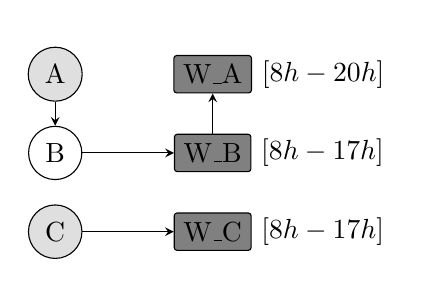
\begin{tikzpicture}
				\node[draw, circle, fill=gray!25, label=above:{$$}] (A)at(-1.5, 0.5) {A};
				\node[draw, circle, label=above:{$$}] (B)at(-1.5, -0.5) {B};
				\node[draw, circle, fill=gray!25, label=above:{$$}] (C)at(-1.5, -1.5) {C};
				\node[draw, rectangle, rounded corners=1pt, fill=gray!100, label=right:{$[8h-20h]$}] (WA)at(0.5, 0.5) {W\_A};
				\node[draw, rectangle, rounded corners=1pt, fill=gray!100, label=right:{$[8h-17h]$}] (WB)at(0.5, -0.5) {W\_B};
				\node[draw, rectangle, rounded corners=1pt, fill=gray!100, label=right:{$[8h-17h]$}] (WC)at(0.5, -1.5) {W\_C};
				\draw[->, >=stealth] (A) -- (B);
				\draw[->, >=stealth] (B) -- (WB);
				\draw[->, >=stealth] (WB) -- (WA);
				\draw[->, >=stealth] (C) -- (WC);
			\end{tikzpicture}
			\caption{Home-to-work trip}
		\end{subfigure}%
		\begin{subfigure}{.5\textwidth}
			\centering
			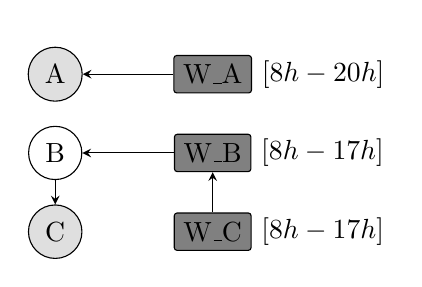
\begin{tikzpicture}
				\node[draw, circle, fill=gray!25, label=above:{$$}] (A)at(-1.5, 0.5) {A};
				\node[draw, circle, label=above:{$$}] (B)at(-1.5, -0.5) {B};
				\node[draw, circle, fill=gray!25, label=above:{$$}] (C)at(-1.5, -1.5) {C};
				\node[draw, rectangle, rounded corners=1pt, fill=gray!100, label=right:{$[8h-20h]$}] (WA)at(0.5, 0.5) {W\_A};
				\node[draw, rectangle, rounded corners=1pt, fill=gray!100, label=right:{$[8h-17h]$}] (WB)at(0.5, -0.5) {W\_B};
				\node[draw, rectangle, rounded corners=1pt, fill=gray!100, label=right:{$[8h-17h]$}] (WC)at(0.5, -1.5) {W\_C};
				\draw[->, >=stealth] (WA) -- (A);
				\draw[->, >=stealth] (WC) -- (WB);
				\draw[->, >=stealth] (WB) -- (B);
				\draw[->, >=stealth] (B) -- (C);
			\end{tikzpicture}
			\caption{Return trip}
		\end{subfigure}
		\caption{Return management}
		\label{fig:Return management}
	\end{figure}
	\end{frame}
	\subsection{Multiple places}
	\begin{frame}
		\frametitle{Originalities}
		\framesubtitle{Multiple places}
		\begin{figure}
		\centering
		\begin{subfigure}{.5\textwidth}
			\centering
			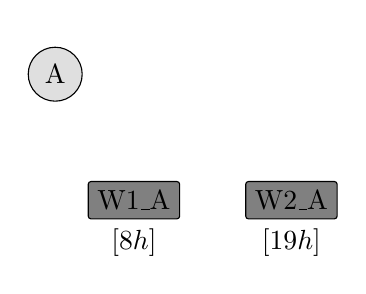
\begin{tikzpicture}
				\node[draw, circle, fill=gray!25, label=above:{$$}] (A)at(-1.5, 1) {A};
				\node[draw, rectangle, rounded corners=1pt, fill=gray!100, label=below:{$[8h]$}] (W1A)at(-0.5, -0.6) {W1\_A};
				\node[draw, rectangle, rounded corners=1pt, fill=gray!100, label=below:{$[19h]$}] (W2A)at(1.5, -0.6) {W2\_A};
			\end{tikzpicture}
			\caption{ Data }
		\end{subfigure}%
		\begin{subfigure}{.5\textwidth}
			\centering
			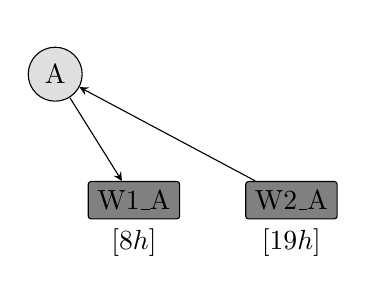
\begin{tikzpicture}
				\node[draw, circle, fill=gray!25, label=above:{$$}] (A)at(-1.5, 1) {A};
				\node[draw, rectangle, rounded corners=1pt, fill=gray!100, label=below:{$[8h]$}] (W1A)at(-0.5, -0.6) {W1\_A};
				\node[draw, rectangle, rounded corners=1pt, fill=gray!100, label=below:{$[19h]$}] (W2A)at(1.5, -0.6) {W2\_A};
				\draw[->, >=stealth, above] (A) -- (W1A) node[midway] {$$};
				\draw[->, >=stealth, above] (W2A) -- (A) node[midway] {$$};
			\end{tikzpicture}
			\caption{ Solution }
		\end{subfigure}
		\caption{Multiple workplaces}
		\label{fig:Several workplaces}
	\end{figure}
	\end{frame}
	\subsection{Waiting time management}
	\begin{frame}
		\frametitle{Originalities}
		\framesubtitle{Waiting time management}
		\begin{figure}
		\centering
		\begin{subfigure}{.5\textwidth}
			\centering
			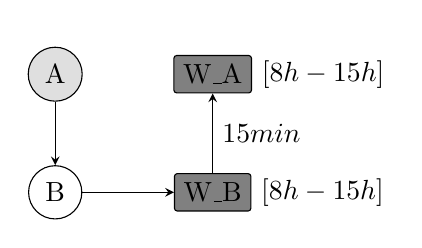
\begin{tikzpicture}
				\node[draw, circle, fill=gray!25, label=above:{$$}] (A)at(-1.5, 1) {A};
				\node[draw, circle, label=above:{$$}] (B)at(-1.5, -0.5) {B};
				\node[draw, rectangle, rounded corners=1pt, fill=gray!100, label=right:{$[8h-15h]$}] (WA)at(0.5, 1) {W\_A};
				\node[draw, rectangle, rounded corners=1pt, fill=gray!100, label=right:{$[8h-15h]$}] (WB)at(0.5, -0.5) {W\_B};
				\draw[->, >=stealth, above] (A) -- (B) node[midway] {$$};
				\draw[->, >=stealth, above] (B) -- (WB) node[midway] {$$};
				\draw[->, >=stealth, right] (WB) -- (WA) node[midway] {$15min$};
			\end{tikzpicture}
			\caption{Allowed advance waiting time = 20 min }
		\end{subfigure}%
		\begin{subfigure}{.5\textwidth}
			\centering
			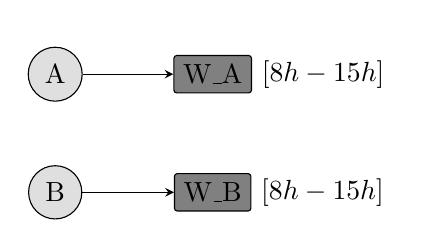
\begin{tikzpicture}
				\node[draw, circle, fill=gray!25, label=above:{$$}] (A)at(-1.5, 1) {A};
				\node[draw, circle, fill=gray!25, label=above:{$$}] (B)at(-1.5, -0.5) {B};
				\node[draw, rectangle, rounded corners=1pt, fill=gray!100, label=right:{$[8h-15h]$}] (WA)at(0.5, 1) {W\_A};
				\node[draw, rectangle, rounded corners=1pt, fill=gray!100, label=right:{$[8h-15h]$}] (WB)at(0.5, -0.5) {W\_B};
				\draw[->, >=stealth, above] (A) -- (WA) node[midway] {$$};
				\draw[->, >=stealth, above] (B) -- (WB) node[midway] {$$};
			\end{tikzpicture}
			\caption{Allowed advance waiting time = 10 min }
		\end{subfigure}
		\caption{Arrival to work waiting time}
		\label{fig:Arrival to work waiting time}
	\end{figure}
	\end{frame}
	\subsection{The case of Grenoble}
	\begin{frame}
		\frametitle{Originalities}
		\framesubtitle{The case of Grenoble}
		\begin{figure}
		\centering
			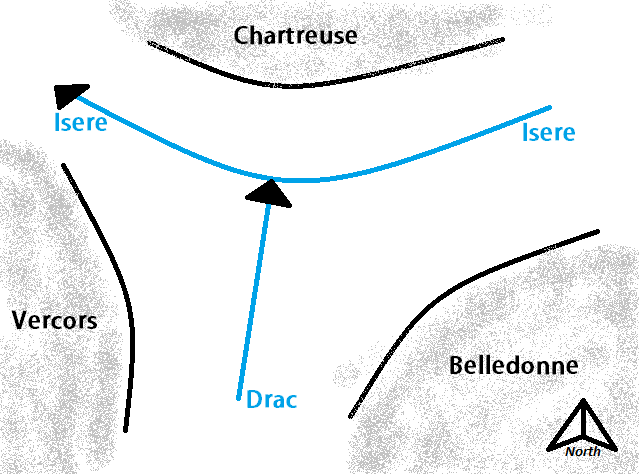
\includegraphics[height=0.5\textwidth]{img/i_grenoble.png}
		\caption{Mountains around Grenoble city}
		\label{fig:Mountains around Grenoble city}
	\end{figure}
	\end{frame}
	%%%%%%%%%%%%%%%% MATHEMATICAL MODEL %%%%%%%%%%
	\section{Modeling}
	\subsection{Data}
	\begin{frame}
		\frametitle{Modeling}
		\framesubtitle{Data}
		\begin{itemize}
		\item $\forall i, j\in V, C_{ij}$ Cost matrices for commuting $arc(i, j)$.
		\item $\forall n\in O, Q_{n}$ Car's capacity of the user $n$. 
		\item $\forall v\in D, B_{v}$ Hour: Beginning of work for the user $n$. 
		\item $\forall v\in K, E_{v}$ Hour: End of work for the user $n$.
		\item $\gamma$ Percentage of the initial travel time added. 
		\item $\delta$ Constant value added to the max travel time. 
		\item $\alpha$ Allowed waiting time to get to work early. 
		\item $\beta$ Allowed waiting time to leave work. 
		\item $M$ A large enough constant. 
	\end{itemize}
	\end{frame}
	\begin{frame}
		\frametitle{Modeling}
		\framesubtitle{Data}
		\begin{figure}
		\centering
			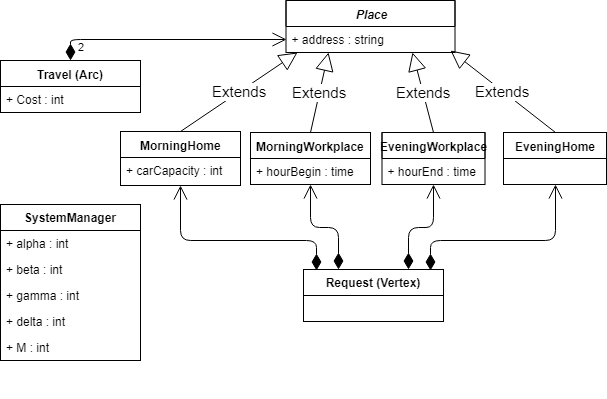
\includegraphics[width=1\textwidth]{img/i_umlproblemdata.png}
		\caption{UML problem diagram}
		\label{fig:UML Diagram}
	\end{figure}
	\end{frame}
	\subsection{Decision variables}
	\begin{frame}
		\frametitle{Modeling}
		\framesubtitle{Decision variables}
		\begin{itemize}
		\item $\forall k\in O, \forall i, j\in V, x^{k}_{ij}=1$ if the travel of the $arc(i, j)$ is deserved by the driver $k$. \\
		\item $\forall k\in O, y^{k}=1$ if the user $k$ is a driver. \\
		\item $\forall k\in O, \forall v\in V, z^{k}_{v}=1$ if the user $k$ is picking or delivering the vertex $v$. \\
		\item $\forall k\in O, \forall v\in V, b^{k}_{v}$ Estimated passage time of the driver $k$ to the vertex $v$. \\
		\item $\forall k\in O, \forall v\in V, q^{k}_{v}$ Number of persons in the car $k$ at the vertex $v$. \\
		\end{itemize}
	\end{frame}
	\subsection{Scheduling}
	\begin{frame}
		\frametitle{Modeling}
		\framesubtitle{Scheduling}
		Sequencing the hours of passages.
	\[ b^{k}_{j}\geq b^{k}_{i}-B_{k+n}+(C_{ij}+B_{k+n})\times x^{k}_{ij}+(B_{k+n}-C_{ij})\times x^{k}_{ji} \]
	\[ b^{k}_{j}\geq b^{k}_{i}-M+(C_{i-2n, j-2n}+M)\times x^{k}_{ij}+(M-C_{i-2n, j-2n})\times x^{k}_{ji} \]
		\footnotetext{Ismail Karaoglan and Fulya Altiparmak. A memetic algorithm for the capacitated
location-routing problem with mixed backhauls. Computers \& Operations
Research, 55:200–216, March 2015.}
		\footnotetext{Hossein Karimi. The capacitated hub covering location-routing problem for simultaneous
pickup and delivery systems. Computers \& Industrial Engineering,
116:47–58, February 2018.}
	\end{frame}
	\subsection{Resolution process}
	\begin{frame}
		\frametitle{Modeling}
		\framesubtitle{Resolution process}
		\begin{figure}
		\centering
			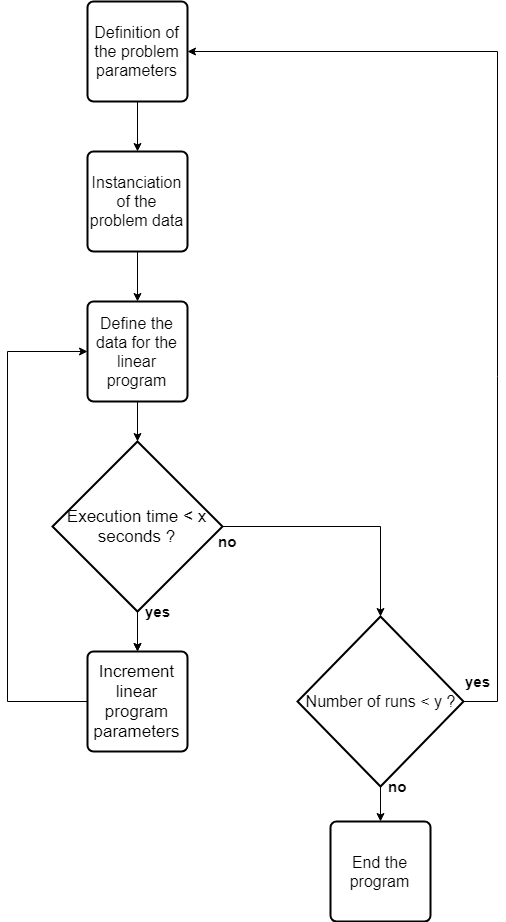
\includegraphics[height=.5\textwidth]{img/i_flowchartlpvariation.png}
		\caption{Flowchart of the LP's parameters variations}
		\label{fig:Flowchart of the LP variations}
	\end{figure}
	\end{frame}
	%%%%%%%%%%%% EXPERIMENTS %%%%%%%%%%%%
	\section{Experiments}
	\subsection{Experimental protocol}
	\begin{frame}
		\frametitle{Experiments}
		\framesubtitle{Experimental protocol}
		The PC used for the experiments:
		\begin{itemize}
		\item Operating System: \textbf{Windows 10 Professional 64-bit version}. 
		\item Code language: \textbf{JAVA }
		\item Solver: \textbf{CPLEX}
		\item RAM quantity: \textbf{8GB}
		\item CPU: \textbf{Intel Core i5-4690 CPU 3.50 GHz}
		\end{itemize}
		 All available at the following web address: \url{https://github.com/NeoKa4ra/CarPoolingInternship}
	\end{frame}
	\subsection{Generator}
	\begin{frame}
		\frametitle{Experiments}
		\framesubtitle{Generator}
		Allowed advance to work: 30 minutes \newline
		Allowed waiting time after job: 15 minutes\newline
		Allowed travel time: $+= 5+20\%$ of the direct trip
	\end{frame}
	
	\subsection{Limits of the model}
	\begin{frame}
		\frametitle{Experiments}
		\framesubtitle{Limits of the model}
		Working hours randomly generated from 8:00 to 9:00 and from 16:00 to 21:00 \newline
		Less than 2\% of GAP on 1 hour for 25 users.\newline
		Less than 10\% of GAP on 1 hour for 30 users.
	\end{frame}
	\subsection{Same and different user pool}
	\begin{frame}
		\frametitle{Experiments}
		\framesubtitle{Difference between same and different user pool}
	\begin{figure}
		\centering
		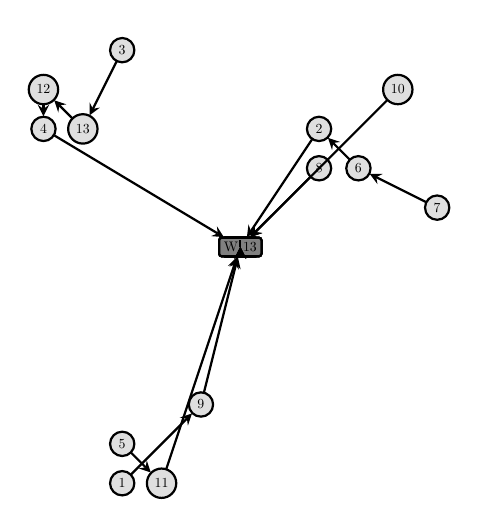
\begin{tikzpicture}[thick,scale=0.5, every node/.style={transform shape}]
			\node[draw,circle,fill=gray!25,label=above:{$$}] (1)at(-3.0,-6.0) {1};
			\node[draw,circle,fill=gray!25,label=above:{$$}] (2)at(2.0,3.0) {2};
			\node[draw,circle,fill=gray!25,label=above:{$$}] (3)at(-3.0,5.0) {3};
			\node[draw,circle,fill=gray!25,label=above:{$$}] (4)at(-5.0,3.0) {4};
			\node[draw,circle,fill=gray!25,label=above:{$$}] (5)at(-3.0,-5.0) {5};
			\node[draw,circle,fill=gray!25,label=above:{$$}] (6)at(3.0,2.0) {6};
			\node[draw,circle,fill=gray!25,label=above:{$$}] (7)at(5.0,1.0) {7};
			\node[draw,circle,fill=gray!25,label=above:{$$}] (8)at(2.0,2.0) {8};
			\node[draw,circle,fill=gray!25,label=above:{$$}] (9)at(-1.0,-4.0) {9};
			\node[draw,circle,fill=gray!25,label=above:{$$}] (10)at(4.0,4.0) {10};
			\node[draw,circle,fill=gray!25,label=above:{$$}] (11)at(-2.0,-6.0) {11};
			\node[draw,circle,fill=gray!25,label=above:{$$}] (12)at(-5.0,4.0) {12};
			\node[draw,circle,fill=gray!25,label=above:{$$}] (13)at(-4.0,3.0) {13};
			\node[draw,rectangle,rounded corners=1pt,fill=gray!100,label=above:{$$}] (W1)at(0.0,0.0) {W\_1};
			\node[draw,rectangle,rounded corners=1pt,fill=gray!100,label=above:{$$}] (W2)at(0.0,0.0) {W\_2};
			\node[draw,rectangle,rounded corners=1pt,fill=gray!100,label=above:{$$}] (W3)at(0.0,0.0) {W\_3};
			\node[draw,rectangle,rounded corners=1pt,fill=gray!100,label=above:{$$}] (W4)at(0.0,0.0) {W\_4};
			\node[draw,rectangle,rounded corners=1pt,fill=gray!100,label=above:{$$}] (W5)at(0.0,0.0) {W\_5};
			\node[draw,rectangle,rounded corners=1pt,fill=gray!100,label=above:{$$}] (W6)at(0.0,0.0) {W\_6};
			\node[draw,rectangle,rounded corners=1pt,fill=gray!100,label=above:{$$}] (W7)at(0.0,0.0) {W\_7};
			\node[draw,rectangle,rounded corners=1pt,fill=gray!100,label=above:{$$}] (W8)at(0.0,0.0) {W\_8};
			\node[draw,rectangle,rounded corners=1pt,fill=gray!100,label=above:{$$}] (W9)at(0.0,0.0) {W\_9};
			\node[draw,rectangle,rounded corners=1pt,fill=gray!100,label=above:{$$}] (W10)at(0.0,0.0) {W\_10};
			\node[draw,rectangle,rounded corners=1pt,fill=gray!100,label=above:{$$}] (W11)at(0.0,0.0) {W\_11};
			\node[draw,rectangle,rounded corners=1pt,fill=gray!100,label=above:{$$}] (W12)at(0.0,0.0) {W\_12};
			\node[draw,rectangle,rounded corners=1pt,fill=gray!100,label=above:{$$}] (W13)at(0.0,0.0) {W\_13};
			\draw[->,>=stealth] (1) -- (9);
			\draw[->,>=stealth] (9) -- (W9);
			\draw[->,>=stealth] (W9) -- (W1);
			\draw[->,>=stealth] (3) -- (13);
			\draw[->,>=stealth] (4) -- (W13);
			\draw[->,>=stealth] (12) -- (4);
			\draw[->,>=stealth] (13) -- (12);
			\draw[->,>=stealth] (W4) -- (W3);
			\draw[->,>=stealth] (W12) -- (W4);
			\draw[->,>=stealth] (W13) -- (W12);
			\draw[->,>=stealth] (5) -- (11);
			\draw[->,>=stealth] (11) -- (W11);
			\draw[->,>=stealth] (W11) -- (W5);
			\draw[->,>=stealth] (2) -- (W6);
			\draw[->,>=stealth] (6) -- (2);
			\draw[->,>=stealth] (7) -- (6);
			\draw[->,>=stealth] (W2) -- (W7);
			\draw[->,>=stealth] (W6) -- (W2);
			\draw[->,>=stealth] (8) -- (W8);
			\draw[->,>=stealth] (10) -- (W10);
		\end{tikzpicture}
		\caption{The same user pool makes the trip to work}
		\label{fig:Graph}
	\end{figure}
	\end{frame}
	\begin{frame}
		\frametitle{Experiments}
		\framesubtitle{Difference between same and different user pool}
\begin{figure}
		\centering
		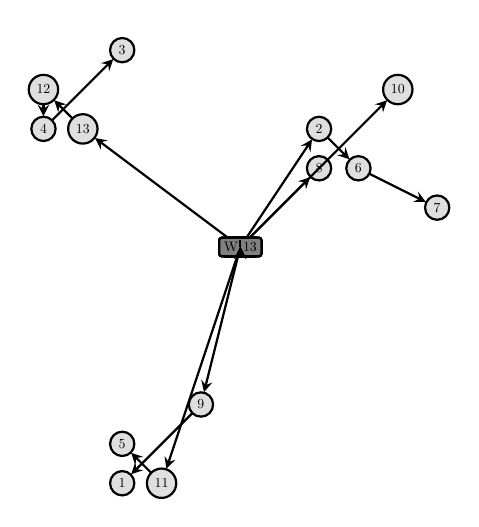
\begin{tikzpicture}[thick,scale=0.5, every node/.style={transform shape}]
			\node[draw,rectangle,rounded corners=1pt,fill=gray!100,label=above:{$$}] (W1)at(0.0,0.0) {W\_1};
			\node[draw,rectangle,rounded corners=1pt,fill=gray!100,label=above:{$$}] (W2)at(0.0,0.0) {W\_2};
			\node[draw,rectangle,rounded corners=1pt,fill=gray!100,label=above:{$$}] (W3)at(0.0,0.0) {W\_3};
			\node[draw,rectangle,rounded corners=1pt,fill=gray!100,label=above:{$$}] (W4)at(0.0,0.0) {W\_4};
			\node[draw,rectangle,rounded corners=1pt,fill=gray!100,label=above:{$$}] (W5)at(0.0,0.0) {W\_5};
			\node[draw,rectangle,rounded corners=1pt,fill=gray!100,label=above:{$$}] (W6)at(0.0,0.0) {W\_6};
			\node[draw,rectangle,rounded corners=1pt,fill=gray!100,label=above:{$$}] (W7)at(0.0,0.0) {W\_7};
			\node[draw,rectangle,rounded corners=1pt,fill=gray!100,label=above:{$$}] (W8)at(0.0,0.0) {W\_8};
			\node[draw,rectangle,rounded corners=1pt,fill=gray!100,label=above:{$$}] (W9)at(0.0,0.0) {W\_9};
			\node[draw,rectangle,rounded corners=1pt,fill=gray!100,label=above:{$$}] (W10)at(0.0,0.0) {W\_10};
			\node[draw,rectangle,rounded corners=1pt,fill=gray!100,label=above:{$$}] (W11)at(0.0,0.0) {W\_11};
			\node[draw,rectangle,rounded corners=1pt,fill=gray!100,label=above:{$$}] (W12)at(0.0,0.0) {W\_12};
			\node[draw,rectangle,rounded corners=1pt,fill=gray!100,label=above:{$$}] (W13)at(0.0,0.0) {W\_13};
			\node[draw,circle,fill=gray!25,label=above:{$$}] (1)at(-3.0,-6.0) {1};
			\node[draw,circle,fill=gray!25,label=above:{$$}] (2)at(2.0,3.0) {2};
			\node[draw,circle,fill=gray!25,label=above:{$$}] (3)at(-3.0,5.0) {3};
			\node[draw,circle,fill=gray!25,label=above:{$$}] (4)at(-5.0,3.0) {4};
			\node[draw,circle,fill=gray!25,label=above:{$$}] (5)at(-3.0,-5.0) {5};
			\node[draw,circle,fill=gray!25,label=above:{$$}] (6)at(3.0,2.0) {6};
			\node[draw,circle,fill=gray!25,label=above:{$$}] (7)at(5.0,1.0) {7};
			\node[draw,circle,fill=gray!25,label=above:{$$}] (8)at(2.0,2.0) {8};
			\node[draw,circle,fill=gray!25,label=above:{$$}] (9)at(-1.0,-4.0) {9};
			\node[draw,circle,fill=gray!25,label=above:{$$}] (10)at(4.0,4.0) {10};
			\node[draw,circle,fill=gray!25,label=above:{$$}] (11)at(-2.0,-6.0) {11};
			\node[draw,circle,fill=gray!25,label=above:{$$}] (12)at(-5.0,4.0) {12};
			\node[draw,circle,fill=gray!25,label=above:{$$}] (13)at(-4.0,3.0) {13};
			\draw[->,>=stealth] (W1) -- (W9);
			\draw[->,>=stealth] (W9) -- (9);
			\draw[->,>=stealth] (9) -- (1);
			\draw[->,>=stealth] (W3) -- (W13);
			\draw[->,>=stealth] (W4) -- (13);
			\draw[->,>=stealth] (W12) -- (W4);
			\draw[->,>=stealth] (W13) -- (W12);
			\draw[->,>=stealth] (4) -- (3);
			\draw[->,>=stealth] (12) -- (4);
			\draw[->,>=stealth] (13) -- (12);
			\draw[->,>=stealth] (W5) -- (W11);
			\draw[->,>=stealth] (W11) -- (11);
			\draw[->,>=stealth] (11) -- (5);
			\draw[->,>=stealth] (W2) -- (2);
			\draw[->,>=stealth] (W6) -- (W2);
			\draw[->,>=stealth] (W7) -- (W6);
			\draw[->,>=stealth] (2) -- (6);
			\draw[->,>=stealth] (6) -- (7);
			\draw[->,>=stealth] (W8) -- (8);
			\draw[->,>=stealth] (W10) -- (10);
		\end{tikzpicture}
		\caption{The same user pool makes the return trip}
		\label{fig:GraphReturn}
	\end{figure}
	\end{frame}
	\begin{frame}
		\frametitle{Experiments}
		\framesubtitle{Difference between same and different user pool}
		Much higher execution time without the same pool. \newline
		5 users : 2.20\% difference ; 10 users : 7.5\% difference.
		\begin{center}
		\captionof{table}{Objective value with 5 users}
		\begin{tabular}{|l|c|r|}
			\hline
			Name of the data & LP & LPSP \\
			\hline
			Mean & 48.96 & 50.04 \\
			Standard deviation & 15.26 & 15.32 \\
			Median & 48.5 & 50.5 \\
			\hline
		\end{tabular}
		\end{center}
		
		\begin{center}
		\captionof{table}{Objective value with 10 users}
		\begin{tabular}{|l|c|r|}
			\hline
			Name of the data & LP & LPSP \\
			\hline
			Mean & 92.00 & 98.90 \\
			Standard deviation & 19.32 & 20.58 \\
			Median & 88.00 & 95.5 \\
			\hline
		\end{tabular}
		\end{center}
	\end{frame}
	
	\subsection{The case of Grenoble}
	\begin{frame}
		\frametitle{Experiments}
		\framesubtitle{The case of Grenoble}
		\begin{figure}
		\centering
		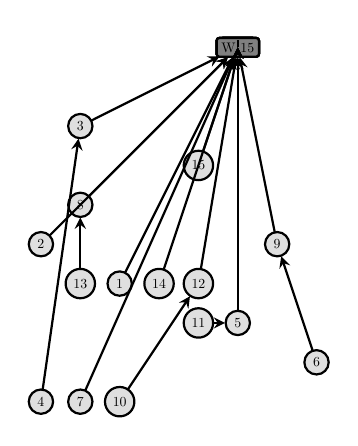
\begin{tikzpicture}[thick,scale=0.5, every node/.style={transform shape}]
			\node[draw,circle,fill=gray!25,label=above:{$$}] (1)at(-3.0,-6.0) {1};
			\node[draw,circle,fill=gray!25,label=above:{$$}] (2)at(-5.0,-5.0) {2};
			\node[draw,circle,fill=gray!25,label=above:{$$}] (3)at(-4.0,-2.0) {3};
			\node[draw,circle,fill=gray!25,label=above:{$$}] (4)at(-5.0,-9.0) {4};
			\node[draw,circle,fill=gray!25,label=above:{$$}] (5)at(0.0,-7.0) {5};
			\node[draw,circle,fill=gray!25,label=above:{$$}] (6)at(2.0,-8.0) {6};
			\node[draw,circle,fill=gray!25,label=above:{$$}] (7)at(-4.0,-9.0) {7};
			\node[draw,circle,fill=gray!25,label=above:{$$}] (8)at(-4.0,-4.0) {8};
			\node[draw,circle,fill=gray!25,label=above:{$$}] (9)at(1.0,-5.0) {9};
			\node[draw,circle,fill=gray!25,label=above:{$$}] (10)at(-3.0,-9.0) {10};
			\node[draw,circle,fill=gray!25,label=above:{$$}] (11)at(-1.0,-7.0) {11};
			\node[draw,circle,fill=gray!25,label=above:{$$}] (12)at(-1.0,-6.0) {12};
			\node[draw,circle,fill=gray!25,label=above:{$$}] (13)at(-4.0,-6.0) {13};
			\node[draw,circle,fill=gray!25,label=above:{$$}] (14)at(-2.0,-6.0) {14};
			\node[draw,circle,fill=gray!25,label=above:{$$}] (15)at(-1.0,-3.0) {15};
			\node[draw,rectangle,rounded corners=1pt,fill=gray!100,label=above:{$$}] (W1)at(0.0,0.0) {W\_1};
			\node[draw,rectangle,rounded corners=1pt,fill=gray!100,label=above:{$$}] (W2)at(0.0,0.0) {W\_2};
			\node[draw,rectangle,rounded corners=1pt,fill=gray!100,label=above:{$$}] (W3)at(0.0,0.0) {W\_3};
			\node[draw,rectangle,rounded corners=1pt,fill=gray!100,label=above:{$$}] (W4)at(0.0,0.0) {W\_4};
			\node[draw,rectangle,rounded corners=1pt,fill=gray!100,label=above:{$$}] (W5)at(0.0,0.0) {W\_5};
			\node[draw,rectangle,rounded corners=1pt,fill=gray!100,label=above:{$$}] (W6)at(0.0,0.0) {W\_6};
			\node[draw,rectangle,rounded corners=1pt,fill=gray!100,label=above:{$$}] (W7)at(0.0,0.0) {W\_7};
			\node[draw,rectangle,rounded corners=1pt,fill=gray!100,label=above:{$$}] (W8)at(0.0,0.0) {W\_8};
			\node[draw,rectangle,rounded corners=1pt,fill=gray!100,label=above:{$$}] (W9)at(0.0,0.0) {W\_9};
			\node[draw,rectangle,rounded corners=1pt,fill=gray!100,label=above:{$$}] (W10)at(0.0,0.0) {W\_10};
			\node[draw,rectangle,rounded corners=1pt,fill=gray!100,label=above:{$$}] (W11)at(0.0,0.0) {W\_11};
			\node[draw,rectangle,rounded corners=1pt,fill=gray!100,label=above:{$$}] (W12)at(0.0,0.0) {W\_12};
			\node[draw,rectangle,rounded corners=1pt,fill=gray!100,label=above:{$$}] (W13)at(0.0,0.0) {W\_13};
			\node[draw,rectangle,rounded corners=1pt,fill=gray!100,label=above:{$$}] (W14)at(0.0,0.0) {W\_14};
			\node[draw,rectangle,rounded corners=1pt,fill=gray!100,label=above:{$$}] (W15)at(0.0,0.0) {W\_15};
			\draw[->,>=stealth] (1) -- (W1);
			\draw[->,>=stealth] (2) -- (W2);
			\draw[->,>=stealth] (3) -- (W3);
			\draw[->,>=stealth] (4) -- (3);
			\draw[->,>=stealth] (W3) -- (W4);
			\draw[->,>=stealth] (6) -- (9);
			\draw[->,>=stealth] (9) -- (W9);
			\draw[->,>=stealth] (W9) -- (W6);
			\draw[->,>=stealth] (7) -- (W7);
			\draw[->,>=stealth] (10) -- (12);
			\draw[->,>=stealth] (12) -- (W12);
			\draw[->,>=stealth] (W12) -- (W10);
			\draw[->,>=stealth] (5) -- (W5);
			\draw[->,>=stealth] (11) -- (5);
			\draw[->,>=stealth] (W5) -- (W11);
			\draw[->,>=stealth] (8) -- (W8);
			\draw[->,>=stealth] (13) -- (8);
			\draw[->,>=stealth] (W8) -- (W13);
			\draw[->,>=stealth] (14) -- (W14);
			\draw[->,>=stealth] (15) -- (W15);
		\end{tikzpicture}
		\caption{Home-to-work: VIZILLE PONT-DE-CLAIX VIF}
	\end{figure}
	\end{frame}
	
	\begin{frame}
		\frametitle{Experiments}
		\framesubtitle{The case of Grenoble}
		\begin{figure}
		\centering
		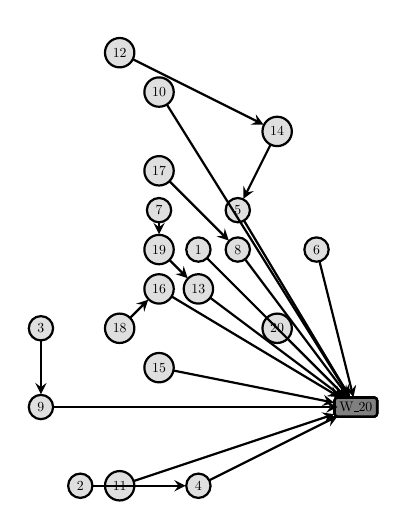
\begin{tikzpicture}[thick,scale=0.5, every node/.style={transform shape}]
			\node[draw,circle,fill=gray!25,label=above:{$$}] (1)at(-4.0,4.0) {1};
			\node[draw,circle,fill=gray!25,label=above:{$$}] (2)at(-7.0,-2.0) {2};
			\node[draw,circle,fill=gray!25,label=above:{$$}] (3)at(-8.0,2.0) {3};
			\node[draw,circle,fill=gray!25,label=above:{$$}] (4)at(-4.0,-2.0) {4};
			\node[draw,circle,fill=gray!25,label=above:{$$}] (5)at(-3.0,5.0) {5};
			\node[draw,circle,fill=gray!25,label=above:{$$}] (6)at(-1.0,4.0) {6};
			\node[draw,circle,fill=gray!25,label=above:{$$}] (7)at(-5.0,5.0) {7};
			\node[draw,circle,fill=gray!25,label=above:{$$}] (8)at(-3.0,4.0) {8};
			\node[draw,circle,fill=gray!25,label=above:{$$}] (9)at(-8.0,0.0) {9};
			\node[draw,circle,fill=gray!25,label=above:{$$}] (10)at(-5.0,8.0) {10};
			\node[draw,circle,fill=gray!25,label=above:{$$}] (11)at(-6.0,-2.0) {11};
			\node[draw,circle,fill=gray!25,label=above:{$$}] (12)at(-6.0,9.0) {12};
			\node[draw,circle,fill=gray!25,label=above:{$$}] (13)at(-4.0,3.0) {13};
			\node[draw,circle,fill=gray!25,label=above:{$$}] (14)at(-2.0,7.0) {14};
			\node[draw,circle,fill=gray!25,label=above:{$$}] (15)at(-5.0,1.0) {15};
			\node[draw,circle,fill=gray!25,label=above:{$$}] (16)at(-5.0,3.0) {16};
			\node[draw,circle,fill=gray!25,label=above:{$$}] (17)at(-5.0,6.0) {17};
			\node[draw,circle,fill=gray!25,label=above:{$$}] (18)at(-6.0,2.0) {18};
			\node[draw,circle,fill=gray!25,label=above:{$$}] (19)at(-5.0,4.0) {19};
			\node[draw,circle,fill=gray!25,label=above:{$$}] (20)at(-2.0,2.0) {20};
			\node[draw,rectangle,rounded corners=1pt,fill=gray!100,label=above:{$$}] (W1)at(0.0,0.0) {W\_1};
			\node[draw,rectangle,rounded corners=1pt,fill=gray!100,label=above:{$$}] (W2)at(0.0,0.0) {W\_2};
			\node[draw,rectangle,rounded corners=1pt,fill=gray!100,label=above:{$$}] (W3)at(0.0,0.0) {W\_3};
			\node[draw,rectangle,rounded corners=1pt,fill=gray!100,label=above:{$$}] (W4)at(0.0,0.0) {W\_4};
			\node[draw,rectangle,rounded corners=1pt,fill=gray!100,label=above:{$$}] (W5)at(0.0,0.0) {W\_5};
			\node[draw,rectangle,rounded corners=1pt,fill=gray!100,label=above:{$$}] (W6)at(0.0,0.0) {W\_6};
			\node[draw,rectangle,rounded corners=1pt,fill=gray!100,label=above:{$$}] (W7)at(0.0,0.0) {W\_7};
			\node[draw,rectangle,rounded corners=1pt,fill=gray!100,label=above:{$$}] (W8)at(0.0,0.0) {W\_8};
			\node[draw,rectangle,rounded corners=1pt,fill=gray!100,label=above:{$$}] (W9)at(0.0,0.0) {W\_9};
			\node[draw,rectangle,rounded corners=1pt,fill=gray!100,label=above:{$$}] (W10)at(0.0,0.0) {W\_10};
			\node[draw,rectangle,rounded corners=1pt,fill=gray!100,label=above:{$$}] (W11)at(0.0,0.0) {W\_11};
			\node[draw,rectangle,rounded corners=1pt,fill=gray!100,label=above:{$$}] (W12)at(0.0,0.0) {W\_12};
			\node[draw,rectangle,rounded corners=1pt,fill=gray!100,label=above:{$$}] (W13)at(0.0,0.0) {W\_13};
			\node[draw,rectangle,rounded corners=1pt,fill=gray!100,label=above:{$$}] (W14)at(0.0,0.0) {W\_14};
			\node[draw,rectangle,rounded corners=1pt,fill=gray!100,label=above:{$$}] (W15)at(0.0,0.0) {W\_15};
			\node[draw,rectangle,rounded corners=1pt,fill=gray!100,label=above:{$$}] (W16)at(0.0,0.0) {W\_16};
			\node[draw,rectangle,rounded corners=1pt,fill=gray!100,label=above:{$$}] (W17)at(0.0,0.0) {W\_17};
			\node[draw,rectangle,rounded corners=1pt,fill=gray!100,label=above:{$$}] (W18)at(0.0,0.0) {W\_18};
			\node[draw,rectangle,rounded corners=1pt,fill=gray!100,label=above:{$$}] (W19)at(0.0,0.0) {W\_19};
			\node[draw,rectangle,rounded corners=1pt,fill=gray!100,label=above:{$$}] (W20)at(0.0,0.0) {W\_20};
			\draw[->,>=stealth] (1) -- (W1);
			\draw[->,>=stealth] (2) -- (4);
			\draw[->,>=stealth] (4) -- (W4);
			\draw[->,>=stealth] (3) -- (9);
			\draw[->,>=stealth] (9) -- (W9);
			\draw[->,>=stealth] (6) -- (W6);
			\draw[->,>=stealth] (7) -- (19);
			\draw[->,>=stealth] (13) -- (W13);
			\draw[->,>=stealth] (19) -- (13);
			\draw[->,>=stealth] (10) -- (W10);
			\draw[->,>=stealth] (11) -- (W11);
			\draw[->,>=stealth] (5) -- (W5);
			\draw[->,>=stealth] (12) -- (14);
			\draw[->,>=stealth] (14) -- (5);
			\draw[->,>=stealth] (15) -- (W15);
			\draw[->,>=stealth] (8) -- (W8);
			\draw[->,>=stealth] (17) -- (8);
			\draw[->,>=stealth] (16) -- (W16);
			\draw[->,>=stealth] (18) -- (16);
			\draw[->,>=stealth] (20) -- (W20);
			\end{tikzpicture}
		\caption{Home-to-work: VOIRON VINAY SAINT-LAURENT-DU-PONT}
	\end{figure}
	\end{frame}
	
	\begin{frame}
		\frametitle{Experiments}
		\framesubtitle{The case of Grenoble}
		\begin{figure}
		\centering
		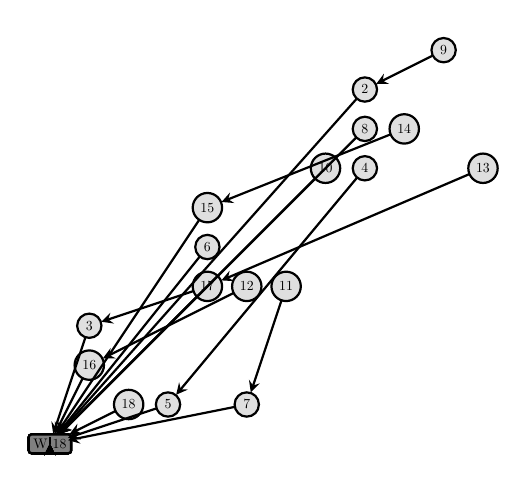
\begin{tikzpicture}[thick,scale=0.5, every node/.style={transform shape}]
			\node[draw,circle,fill=gray!25,label=above:{$$}] (1)at(4.0,4.0) {1};
			\node[draw,circle,fill=gray!25,label=above:{$$}] (2)at(8.0,9.0) {2};
			\node[draw,circle,fill=gray!25,label=above:{$$}] (3)at(1.0,3.0) {3};
			\node[draw,circle,fill=gray!25,label=above:{$$}] (4)at(8.0,7.0) {4};
			\node[draw,circle,fill=gray!25,label=above:{$$}] (5)at(3.0,1.0) {5};
			\node[draw,circle,fill=gray!25,label=above:{$$}] (6)at(4.0,5.0) {6};
			\node[draw,circle,fill=gray!25,label=above:{$$}] (7)at(5.0,1.0) {7};
			\node[draw,circle,fill=gray!25,label=above:{$$}] (8)at(8.0,8.0) {8};
			\node[draw,circle,fill=gray!25,label=above:{$$}] (9)at(10.0,10.0) {9};
			\node[draw,circle,fill=gray!25,label=above:{$$}] (10)at(7.0,7.0) {10};
			\node[draw,circle,fill=gray!25,label=above:{$$}] (11)at(6.0,4.0) {11};
			\node[draw,circle,fill=gray!25,label=above:{$$}] (12)at(5.0,4.0) {12};
			\node[draw,circle,fill=gray!25,label=above:{$$}] (13)at(11.0,7.0) {13};
			\node[draw,circle,fill=gray!25,label=above:{$$}] (14)at(9.0,8.0) {14};
			\node[draw,circle,fill=gray!25,label=above:{$$}] (15)at(4.0,6.0) {15};
			\node[draw,circle,fill=gray!25,label=above:{$$}] (16)at(1.0,2.0) {16};
			\node[draw,circle,fill=gray!25,label=above:{$$}] (17)at(4.0,4.0) {17};
			\node[draw,circle,fill=gray!25,label=above:{$$}] (18)at(2.0,1.0) {18};
			\node[draw,rectangle,rounded corners=1pt,fill=gray!100,label=above:{$$}] (W1)at(0.0,0.0) {W\_1};
			\node[draw,rectangle,rounded corners=1pt,fill=gray!100,label=above:{$$}] (W2)at(0.0,0.0) {W\_2};
			\node[draw,rectangle,rounded corners=1pt,fill=gray!100,label=above:{$$}] (W3)at(0.0,0.0) {W\_3};
			\node[draw,rectangle,rounded corners=1pt,fill=gray!100,label=above:{$$}] (W4)at(0.0,0.0) {W\_4};
			\node[draw,rectangle,rounded corners=1pt,fill=gray!100,label=above:{$$}] (W5)at(0.0,0.0) {W\_5};
			\node[draw,rectangle,rounded corners=1pt,fill=gray!100,label=above:{$$}] (W6)at(0.0,0.0) {W\_6};
			\node[draw,rectangle,rounded corners=1pt,fill=gray!100,label=above:{$$}] (W7)at(0.0,0.0) {W\_7};
			\node[draw,rectangle,rounded corners=1pt,fill=gray!100,label=above:{$$}] (W8)at(0.0,0.0) {W\_8};
			\node[draw,rectangle,rounded corners=1pt,fill=gray!100,label=above:{$$}] (W9)at(0.0,0.0) {W\_9};
			\node[draw,rectangle,rounded corners=1pt,fill=gray!100,label=above:{$$}] (W10)at(0.0,0.0) {W\_10};
			\node[draw,rectangle,rounded corners=1pt,fill=gray!100,label=above:{$$}] (W11)at(0.0,0.0) {W\_11};
			\node[draw,rectangle,rounded corners=1pt,fill=gray!100,label=above:{$$}] (W12)at(0.0,0.0) {W\_12};
			\node[draw,rectangle,rounded corners=1pt,fill=gray!100,label=above:{$$}] (W13)at(0.0,0.0) {W\_13};
			\node[draw,rectangle,rounded corners=1pt,fill=gray!100,label=above:{$$}] (W14)at(0.0,0.0) {W\_14};
			\node[draw,rectangle,rounded corners=1pt,fill=gray!100,label=above:{$$}] (W15)at(0.0,0.0) {W\_15};
			\node[draw,rectangle,rounded corners=1pt,fill=gray!100,label=above:{$$}] (W16)at(0.0,0.0) {W\_16};
			\node[draw,rectangle,rounded corners=1pt,fill=gray!100,label=above:{$$}] (W17)at(0.0,0.0) {W\_17};
			\node[draw,rectangle,rounded corners=1pt,fill=gray!100,label=above:{$$}] (W18)at(0.0,0.0) {W\_18};
			\draw[->,>=stealth] (1) -- (W1);
			\draw[->,>=stealth] (4) -- (5);
			\draw[->,>=stealth] (5) -- (W5);
			\draw[->,>=stealth] (W5) -- (W4);
			\draw[->,>=stealth] (6) -- (W6);
			\draw[->,>=stealth] (8) -- (W8);
			\draw[->,>=stealth] (2) -- (W2);
			\draw[->,>=stealth] (9) -- (2);
			\draw[->,>=stealth] (W2) -- (W9);
			\draw[->,>=stealth] (10) -- (W10);
			\draw[->,>=stealth] (7) -- (W7);
			\draw[->,>=stealth] (11) -- (7);
			\draw[->,>=stealth] (W7) -- (W11);
			\draw[->,>=stealth] (12) -- (16);
			\draw[->,>=stealth] (16) -- (W16);
			\draw[->,>=stealth] (W16) -- (W12);
			\draw[->,>=stealth] (3) -- (W3);
			\draw[->,>=stealth] (13) -- (17);
			\draw[->,>=stealth] (17) -- (3);
			\draw[->,>=stealth] (W3) -- (W17);
			\draw[->,>=stealth] (W17) -- (W13);
			\draw[->,>=stealth] (14) -- (15);
			\draw[->,>=stealth] (15) -- (W15);
			\draw[->,>=stealth] (W15) -- (W14);
			\draw[->,>=stealth] (18) -- (W18);
			\end{tikzpicture}
		\caption{Home-to-work: PONTCHARRA LE-TOUVET CROLLES}
		\label{fig:Return trip for the cities : PONTCHARRA LE-TOUVET CROLLES}
	\end{figure}
	\end{frame}
	%%%%%%%%%%%%%%%% CONCLUSION %%%%%%%%%%%%
	\section*{Conclusion}
	\begin{frame}
		\frametitle{Conclusion}
		Thank you for listening
	\end{frame}
\end{document}